\begin{frame}
  \frametitle{Vullen van vierkanten}
  \framesubtitle{Resultaten: vullen van een vierkant met kleinere vierkanten}
  \begin{columns}
    \begin{column}{0.5\textwidth}
      \definecolor{cqcqcq}{rgb}{0.75,0.75,0.75}
\begin{tikzpicture}[scale=0.4,line cap=round,line join=round,>=triangle 45,x=1.0cm,y=1.0cm]
\draw [color=cqcqcq,dash pattern=on 2pt off 2pt, xstep=1.0cm,ystep=1.0cm] (-0.5,-0.5) grid (10.5,10.5);
\clip(-0.5,-0.5) rectangle (10.5,10.5);
\filldraw[line width=1.6pt,fill=black,fill opacity=0.1] (0,0) -- (10,0) -- (10,10) -- (0,10) -- cycle;
\filldraw[fill=black,fill opacity=0.1] (0,0) -- (3,0) -- (3,3) -- (0,3) -- cycle;
\filldraw[fill=black,fill opacity=0.1] (3,0) -- (6,0) -- (6,3) -- (3,3) -- cycle;
\filldraw[fill=black,fill opacity=0.1] (6,0) -- (9,0) -- (9,3) -- (6,3) -- cycle;
\filldraw[fill=black,fill opacity=0.1] (0,3) -- (3,3) -- (3,6) -- (0,6) -- cycle;
\filldraw[fill=black,fill opacity=0.1] (3,3) -- (6,3) -- (6,6) -- (3,6) -- cycle;
\filldraw[fill=black,fill opacity=0.1] (6,3) -- (9,3) -- (9,6) -- (6,6) -- cycle;
\filldraw[fill=black,fill opacity=0.1] (0,6) -- (3,6) -- (3,9) -- (0,9) -- cycle;
\filldraw[fill=black,fill opacity=0.1] (3,6) -- (6,6) -- (6,9) -- (3,9) -- cycle;
\filldraw[fill=black,fill opacity=0.1] (6,6) -- (9,6) -- (9,9) -- (6,9) -- cycle;
\end{tikzpicture}

    \end{column}
    \begin{column}{0.5\textwidth}
    \begin{itemize}
      \item Voorbeeld:
      \begin{align*}
        10^2  &= (3\cdot 3 + 1)^2\\
        \Leftrightarrow 100   &= (3\cdot 3)^2 + 2\cdot 3\cdot 3\cdot 1 + 1^2\\
        \Leftrightarrow 100   &= 81 + 19
      \end{align*}
      \pause
      \item Algemeen:
      \begin{align*}
         a^2  &= (q\cdot d + r)^2\\
        \Leftrightarrow a^2   &= (q\cdot d)^2 + 2\cdot q\cdot d\cdot r + r^2
      \end{align*}
      {\tiny met $a$ de zijde van het grote vierkante, $d$ de zijde van de kleine vierkanten, $q$ het aantal keer we $d$ in $a$ krijgen en $r$ de rest die dan nog overblijft}
    \end{itemize}
    \end{column}
  \end{columns}  
\end{frame}

\begin{frame}
  \frametitle{Vullen van vierkanten}
  \framesubtitle{Alles over perfecte vierkanten}
  \begin{columns}
    \begin{column}{0.4\textwidth}
      \only<1-3>{{\small
\begin{tikzpicture}[scale=0.04,line cap=round,line join=round,>=triangle 45,x=1.0cm,y=1.0cm]
\clip(-0.5,-0.5) rectangle (113,113);
\filldraw[fill=black,fill opacity=0.05] (0,0) -- (33,0) -- (33,33) -- (0,33) -- cycle;
\filldraw[fill=black,fill opacity=0.05] (33,0) -- (70,0) -- (70,37) -- (33,37) -- cycle;
\filldraw[fill=black,fill opacity=0.05] (70,0) -- (112,0) -- (112,42) -- (70,42) -- cycle;
\filldraw[fill=black,fill opacity=0.05] (0,33) -- (29,33) -- (29,62) -- (0,62) -- cycle;
\filldraw[fill=black,fill opacity=0.05] (29,33) -- (33,33) -- (33,37) -- (29,37) -- cycle;
\filldraw[fill=black,fill opacity=0.05] (0,62) -- (50,62) -- (50,112) -- (0,112) -- cycle;
\filldraw[fill=black,fill opacity=0.05] (29,62) -- (29,37) -- (54,37) -- (54,62) -- cycle;
\filldraw[fill=black,fill opacity=0.05] (54,37) -- (70,37) -- (70,53) -- (54,53) -- cycle;
\filldraw[fill=black,fill opacity=0.05] (70,42) -- (88,42) -- (88,60) -- (70,60) -- cycle;
\filldraw[fill=black,fill opacity=0.05] (88,42) -- (112,42) -- (112,66) -- (88,66) -- cycle;
\filldraw[fill=black,fill opacity=0.05] (54,53) -- (63,53) -- (63,62) -- (54,62) -- cycle;
\filldraw[fill=black,fill opacity=0.05] (63,53) -- (70,53) -- (70,60) -- (63,60) -- cycle;
\filldraw[fill=black,fill opacity=0.05] (63,60) -- (65,60) -- (65,62) -- (63,62) -- cycle;
\filldraw[fill=black,fill opacity=0.05] (82,60) -- (88,60) -- (88,66) -- (82,66) -- cycle;
\filldraw[fill=black,fill opacity=0.05] (65,60) -- (82,60) -- (82,77) -- (65,77) -- cycle;
\filldraw[fill=black,fill opacity=0.05] (50,62) -- (65,62) -- (65,77) -- (50,77) -- cycle;
\filldraw[fill=black,fill opacity=0.05] (50,112) -- (50,77) -- (85,77) -- (85,112) -- cycle;
\filldraw[fill=black,fill opacity=0.05] (82,77) -- (82,66) -- (93,66) -- (93,77) -- cycle;
\filldraw[fill=black,fill opacity=0.05] (93,66) -- (112,66) -- (112,85) -- (93,85) -- cycle;
\filldraw[fill=black,fill opacity=0.05] (85,77) -- (93,77) -- (93,85) -- (85,85) -- cycle;
\filldraw[fill=black,fill opacity=0.05] (85,85) -- (112,85) -- (112,112) -- (85,112) -- cycle;
\end{tikzpicture}
}
}
      \only<4>{{\small
\begin{tikzpicture}[scale=0.04,line cap=round,line join=round,>=triangle 45,x=1.0cm,y=1.0cm]
\clip(-0.5,-0.5) rectangle (113,113);
\filldraw[fill=black,fill opacity=0.05] (0,0) -- (33,0) -- (33,33) -- (0,33) -- cycle;
\filldraw[fill=black,fill opacity=0.05] (33,0) -- (70,0) -- (70,37) -- (33,37) -- cycle;
\filldraw[fill=black,fill opacity=0.05] (70,0) -- (112,0) -- (112,42) -- (70,42) -- cycle;
\filldraw[fill=black,fill opacity=0.05] (0,33) -- (29,33) -- (29,62) -- (0,62) -- cycle;
\filldraw[fill=black,fill opacity=0.05] (29,33) -- (33,33) -- (33,37) -- (29,37) -- cycle;
\filldraw[fill=black,fill opacity=0.05] (0,62) -- (50,62) -- (50,112) -- (0,112) -- cycle;
\filldraw[fill=black,fill opacity=0.05] (29,62) -- (29,37) -- (54,37) -- (54,62) -- cycle;
\filldraw[fill=black,fill opacity=0.05] (54,37) -- (70,37) -- (70,53) -- (54,53) -- cycle;
\filldraw[fill=black,fill opacity=0.05] (70,42) -- (88,42) -- (88,60) -- (70,60) -- cycle;
\filldraw[fill=black,fill opacity=0.05] (88,42) -- (112,42) -- (112,66) -- (88,66) -- cycle;
\filldraw[fill=black,fill opacity=0.05] (54,53) -- (63,53) -- (63,62) -- (54,62) -- cycle;
\filldraw[fill=black,fill opacity=0.05] (63,53) -- (70,53) -- (70,60) -- (63,60) -- cycle;
\filldraw[fill=black,fill opacity=0.5] (63,60) -- (65,60) -- (65,62) -- (63,62) -- cycle;
\filldraw[fill=black,fill opacity=0.05] (82,60) -- (88,60) -- (88,66) -- (82,66) -- cycle;
\filldraw[fill=black,fill opacity=0.05] (65,60) -- (82,60) -- (82,77) -- (65,77) -- cycle;
\filldraw[fill=black,fill opacity=0.05] (50,62) -- (65,62) -- (65,77) -- (50,77) -- cycle;
\filldraw[fill=black,fill opacity=0.05] (50,112) -- (50,77) -- (85,77) -- (85,112) -- cycle;
\filldraw[fill=black,fill opacity=0.05] (82,77) -- (82,66) -- (93,66) -- (93,77) -- cycle;
\filldraw[fill=black,fill opacity=0.05] (93,66) -- (112,66) -- (112,85) -- (93,85) -- cycle;
\filldraw[fill=black,fill opacity=0.05] (85,77) -- (93,77) -- (93,85) -- (85,85) -- cycle;
\filldraw[fill=black,fill opacity=0.05] (85,85) -- (112,85) -- (112,112) -- (85,112) -- cycle;
\end{tikzpicture}
}
}
    \end{column}
    \begin{column}{0.6\textwidth}
    {\scriptsize
      \begin{itemize}
        \item Een {\bf perfect vierkant} is een vierkant dat opgedeeld kan worden in een eindig aantal kleinere vierkanten waarvan geen twee dezelfde grootte hebben.
        \item De {\bf orde} van een perfect vierkant is het aantal kleinere vierkanten dat het bevat.
        \pause
        \item Het vierkant heeft $8$ symmetriën, de dihedrale groep $D4$, dus één oplossing leidt tot 8 isomorfe oplossingen.
          \begin{center}
            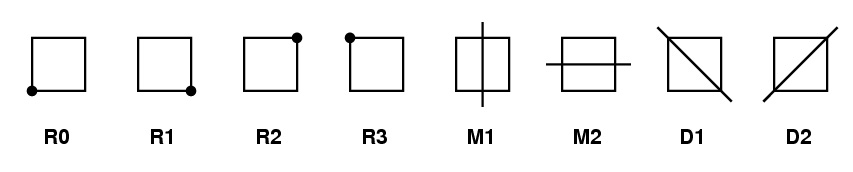
\includegraphics[width=0.8\textwidth]{dih4}
          \end{center}
        \pause
        \item Door het perfecte vierkant te hertekenen binnen het kleinste vierkantje construeren we nieuwe perfecte vierkanten.
        \item Een {\bf fractaal} is een meetkundige figuur die zelfgelijkend is. 
      \end{itemize}
    }
    \end{column}
  \end{columns}  
\end{frame}

\begin{frame}
  \frametitle{Vullen van vierkanten}
  \framesubtitle{Eigenschap kleinste vierkantje in een perfect vierkant}
  \begin{columns}
    \begin{column}{0.5\textwidth}
      %\only<1>{\definecolor{cccccc}{rgb}{0.6,0.6,0.6}
\begin{tikzpicture}[scale=0.3, line cap=round,line join=round,>=triangle 45,x=1.0cm,y=1.0cm]
\clip(45,32) rectangle (75,61);
\draw [line width=1.2pt, color=cccccc] (65,32) -- (65,61);
\filldraw[line width=1.2pt,fill=black,fill opacity=0.1] (54,59.12) -- (63,59.12) -- (63,50.12) -- (54,50.12) -- cycle;
\filldraw[line width=1.2pt,fill=black,fill opacity=0.1] (63,59.12) -- (70,59.12) -- (70,52.12) -- (63,52.12) -- cycle;
\filldraw[line width=1.2pt,fill=black,fill opacity=0.15] (63,52.12) -- (65,52.12) -- (65,50.12) -- (63,50.12) -- cycle;
\filldraw[line width=1.2pt,fill=black,fill opacity=0.1] (50,50.12) -- (65,50.12) -- (65,35.12) -- (50,35.12) -- cycle;
\end{tikzpicture}
}
      \definecolor{cccccc}{rgb}{0.6,0.6,0.6}
\begin{tikzpicture}[scale=0.3, line cap=round,line join=round,>=triangle 45,x=1.0cm,y=1.0cm]
\clip(45,32) rectangle (75,61);
\draw [line width=1.2pt, color=cccccc] (65,32) -- (65,61);
\filldraw[line width=1.2pt,fill=black,fill opacity=0.1] (54,59.12) -- (63,59.12) -- (63,50.12) -- (54,50.12) -- cycle;
\filldraw[line width=1.2pt,fill=black,fill opacity=0.1] (63,59.12) -- (70,59.12) -- (70,52.12) -- (63,52.12) -- cycle;
\filldraw[line width=1.2pt,fill=black,fill opacity=0.15] (63,52.12) -- (65,52.12) -- (65,50.12) -- (63,50.12) -- cycle;
\filldraw[line width=1.2pt,fill=black,fill opacity=0.1] (50,50.12) -- (65,50.12) -- (65,35.12) -- (50,35.12) -- cycle;
\end{tikzpicture}

    \end{column}
    \begin{column}{0.5\textwidth}
    {\scriptsize
      \begin{stelling}
      Het kleinste vierkantje in een perfect vierkant kan nooit aan de rand liggen.
      \end{stelling}
      {\tiny
        \begin{list}{}{\leftmargin=0pt}
          \pause
          \item Uit het ongerijmde.
          \item Veronderstel dat het kleinste vierkantje in een perfect vierkant op de rand ligt.
          \pause
          \item Hoeveel vierkantjes liggen dan nog rond het kleinste vierkantje?
          \item Wat weten we over de vierkantjes die rond het kleinste vierkantje liggen?
          \pause
          \item Dus één van de vierkantjes komt over de rand!
          \pause
          \item Dus we hebben geen perfect vierkant, een strijdigheid!
          \item Dus het kleinste vierkantje kan niet op de rand liggen!
        \end{list}
      }
    }
    \end{column}
  \end{columns}  
\end{frame}

